\documentclass[a4paper,14pt]{extarticle}
\usepackage{../../tex-shared/report-layout}

\begin{document}
\begin{titlepage}
    
    \thispagestyle{empty}
    
    \begin{center}
        
        Министерство науки и Высшего образования Российской Федерации \\
        Севастопольский государственный университет \\
        Кафедра ИС
        
        \vfill

        Отчет \\
        по лабораторной работе №\mylabnumber \\
        \enquote{\mylabtitle} \\
        по дисциплине \\
        \enquote{\MakeTextUppercase{\mysubject}}

    \end{center}

    \vspace{1cm}

    \noindent\hspace{7.5cm} Выполнил студент группы ИС/б-17-2-о \\
    \null\hspace{7.5cm} Горбенко К. Н. \\
    \null\hspace{7.5cm} Проверил \\
    \null\hspace{7.5cm} \mylecturer

    \vfill

    \begin{center}
        Севастополь \\
        \the\year{}
    \end{center}

\end{titlepage}

\section*{Введение}
На сегодняшний день, при разработке программного обеспечения важно помнить о
том, что начинать её следует с проектирования — т.е. с полного планирования
того, что непосредственно нам придётся разрабатывать, в какие сроки, с какими
исходными данными и ожидаемым результатом. Отсутствие подобной практики перед
разработкой влечет за собой проблемы в будущем в виде отсутствия понимания
структуры ПО.

Целью данной расчётно-графической работы является проектирование
предметной области \enquote{Сервис для помощи в изучении иностранной лексики}.
Для реализации данной работы, были проведены следующие этапы:
\begin{itemize}
    \item исследование и
          функциональное моделирование процессов при помощи DFD, IDEF0, IDEF1X, IDEF3,
          BPMN диаграмм;
    \item выбор и применение инструментального средства для
          функционального моделирования потоков данных и процессов, построения реляционных
          информационных структур, описания логики взаимодействия информационных потоков и
          моделирования бизнес-процессов.
\end{itemize}

\section{Описание предметной области и нотаций}
\subsection{Предметная область}
Предметная область -- сервис для изучения лексики английского языка.
Единственным действующим лицом является пользователь. Пользователю доступны
следующие базовые функции:
\begin{enumerate}
    \item создание групп словарей;
    \item создание словарей;
    \item создание переводов внутри словарей (импорт из внешних словарей с
          возможностью редактирования импортированной информации), добавление
          расширенного описания к переводу (флэш-карточки);
    \item получение списков групп словарей, списков словарей, списков переводов;
    \item редактирование перевода и его описания;
    \item предоставление доступа к пользовательским словарям другим пользователям;
    \item экспорт/импорт словарей;
    \item получение списка упражнений и решение этих упражнений (для словаря,
          для группы словарей, для всех словарей).
\end{enumerate}

\subsection{Описание нотаций}
\subsubsection{DFD}
\textbf{DFD} – общепринятое сокращение от англ. data flow diagrams — диаграммы потоков
данных. Так называется методология графического структурного анализа,
описывающая внешние по отношению к системе источники и адресаты данных,
логические функции, потоки данных и хранилища данных, к которым осуществляется
доступ.

\subsubsection{IDEF0}
\textbf{IDEF0} – методология функционального моделирования. С помощью наглядного
графического языка IDEF0 изучаемая система предстаёт перед разработчиками и
аналитиками в виде набора взаимосвязанных функций (функциональных блоков — в
терминах IDEF0). Как правило, моделирование средствами IDEF0 является первым
этапом изучения любой системы.

\subsubsection{IDEF1X}
\textbf{IDEF1X} – методология моделирования баз данных на основе модели \\\enquote{сущность-связь}.
Применяется для построения информационной модели, которая представляет структуру
информации, необходимой для поддержки функций производственной системы или
среды. Метод IDEF1, разработанный Т. Рэйми (T. Ramey) на основе подходов П. Чена
и позволяет построить модель данных, эквивалентную реляционной модели в третьей
нормальной форме. В настоящее время на основе совершенствования методологии
IDEF1 создана её новая версия — методология IDEF1X. Она разработана с учётом
таких требований, как простота изучения и возможность автоматизации.

\subsubsection{IDEF3}
\textbf{IDEF3} – методология документирования процессов, происходящих в системе
(например, на предприятии), описывает сценарий и последовательность операций для
каждого процесса. IDEF3 имеет прямую взаимосвязь с методологией IDEF0 — каждая
функция (функциональный блок) может быть представлена в виде отдельного процесса
средствами IDEF3.

\subsubsection{BPMN}
\textbf{BPMN} – описывает условные обозначения и их описание в XML для отображения
бизнес-процессов в виде диаграмм бизнес-процессов. BPMN ориентирована как на
технических специалистов, так и на бизнес-пользователей. Для этого язык
использует базовый набор интуитивно понятных элементов, которые позволяют
определять сложные семантические конструкции. Кроме того, спецификация BPMN
определяет, как диаграммы, описывающие бизнес-процесс, могут быть
трансформированы в исполняемые модели.

В данном разделе была описана предметная область и выполнено описание нотаций,
диаграммы которых буду построены в следующем пункте.

\section{Выполнение}
\subsection{Выбор инструментальных средств}
\subsubsection{RamusEducational}
Для моделирования потоков данных и процессов была использована программа Ramus
Education. Ramus Education может быть использован для создания диаграмм в
формате IDEF0 и DFD. Ramus Education использует формат файлов полностью
совместимый с форматом файла коммерческой версии Ramus. Как и Ramus, Ramus
Educational поддерживает импорт/экспорт файлов в формат IDL, таким образом,
реализуя частичную совместимость с подобными программами (например, с CA Erwin
Process Modeler). Ramus Educational доступен только в локальном варианте, и
ограничен по функциональности. Перечень основных ограничений по сравнению с
коммерческой локальной версией: - ограничен перечень доступных атрибутов
классификаторов; - отсутствует функциональность для работы с матричными
проекциями классификаторов; - отсутствует редактор отчётов; - отсутствует
навигатор по модели. Ramus Educational поддерживает единый формат файлов с
локальной версией Ramus. Файл созданный в Ramus Educational можно редактировать
в локальной версии Ramus и наоборот. Также имеется возможность импорта/экспорта
файлов в формат IDL BPWin. Обеспечивается частичная совместимость с CA ERwin
Process Modeler (в части графических моделей IDEF0).

\subsubsection{CA ERwin Data Modeler Community Edition}
Выполнения построения IDEF1X и IDEF3 диаграмм осуществлено при помощи
CASE-средства CA ERwin Data Modeler Community Edition - лидер среди
проприетарных CASE-средств поддержки методологий информационного моделирования.
Бесплатное базовое средство моделирования CA ERwin Data Modeler Community
Edition включает в себя подмножество функций флагманского продукта.

\subsubsection{ARIS Business Performance Edition}
Из наиболее популярных зарубежных программных продуктов для моделирования бизнес
процессов выделяются:
\begin{itemize}
    \item ARIS Business Performance Edition;
    \item CA ERwin Data Modeler;
    \item Hyperion Performance Scorecard;
    \item IBM WebSphere Business Modeler;
    \item SAP Strategic Enterprise Management (SAP).
\end{itemize}

Наиболее мощной из представленных выше систем и самой дорогой является
инструментальная система ARIS, которая представляет собой интегрированное
семейство программных продуктов, предназначенных для структурированного
описания, анализа и последующего совершенствования бизнес процессов предприятия,
а также подготовки организаций к внедрению сложных информационных систем.

Всемногообразие программных продуктов ARIS можно разделить на четыре платформы,
одна из которых поддерживает разработку стратегии организации, а три остальных
соответствуют основным этапам жизненного цикла системы управления.

В совокупности четыре специализированных модуля образуют единую интегрированную
систему, направленную на поддержание полного цикла управления бизнес-процессами.


Хоть Ramus Education, CA ERwin Data Modeler Community Edition, ARIS Business
Performance Edition и имеют некоторые недостатки в виде ограниченного
функционала (бесплатных версий), однако доступного набора возможностей
достаточно чтобы построить диаграммы в формате IDEF0, DFD, IDEF1X, IDEF3 и
моделировать процессы в системе для текущего варианта.

\subsection{Построение диаграмм}
\subsubsection{DFD}
На рисунке \ref{fig:main-process} изображена \code{DFD}-диаграмма основного
процесса системы:

\begin{figure}[H]
    \centering
    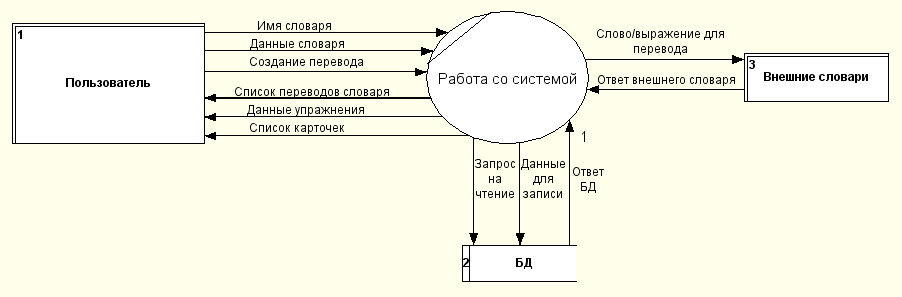
\includegraphics[width=\linewidth]{main-process}
    \caption{\code{DFD}-диаграмма основного процесса системы}
    \label{fig:main-process}
\end{figure}

На рисунке \ref{fig:translation-creation-process} изображена
\code{DFD}-диаграмма процесса создания перевода:

\begin{figure}[H]
    \centering
    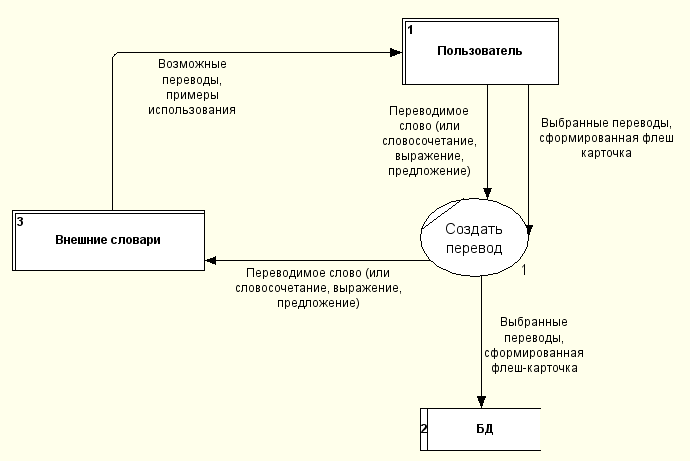
\includegraphics[width=\linewidth]{translation-creation-process}
    \caption{\code{DFD}-диаграмма процесса создания перевода}
    \label{fig:translation-creation-process}
\end{figure}

На рисунке \ref{fig:excercise-receival-process} изображена \code{DFD}-диаграмма
процесса получения упражнений:

\begin{figure}[H]
    \centering
    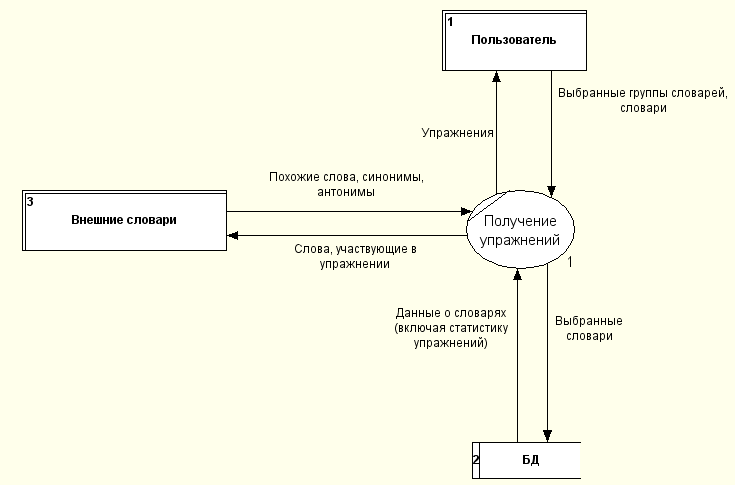
\includegraphics[width=\linewidth]{excercise-receival-process}
    \caption{\code{DFD}-диаграмма процесса получения упражнений}
    \label{fig:excercise-receival-process}
\end{figure}

\subsubsection{IDEF0}
Составим контекстную диаграмму основного процесса (рисунок \ref{fig:context-diagram}) в
нотации \code{IDEF0}.

\begin{figure}[H]
    \centering
    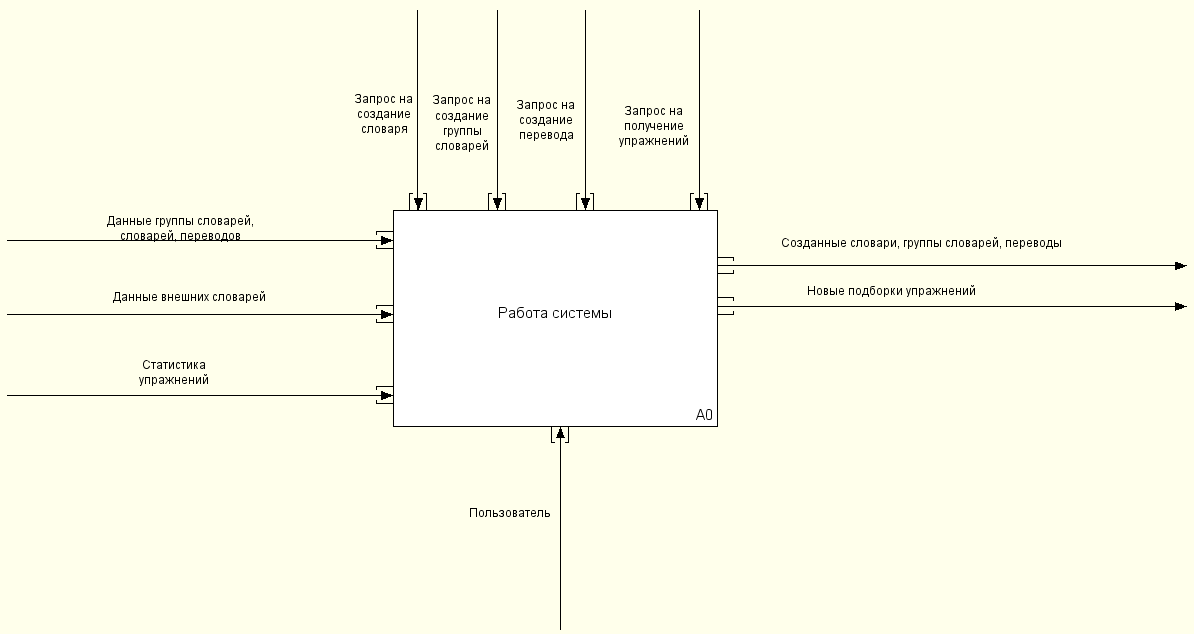
\includegraphics[width=\linewidth]{context-diagram}
    \caption{Контекстная диаграмма основного процесса системы}
    \label{fig:context-diagram}
\end{figure}

На рисунке \ref{fig:tree} изображена диаграмма дерева узлов системы.
\begin{figure}[H]
    \centering
    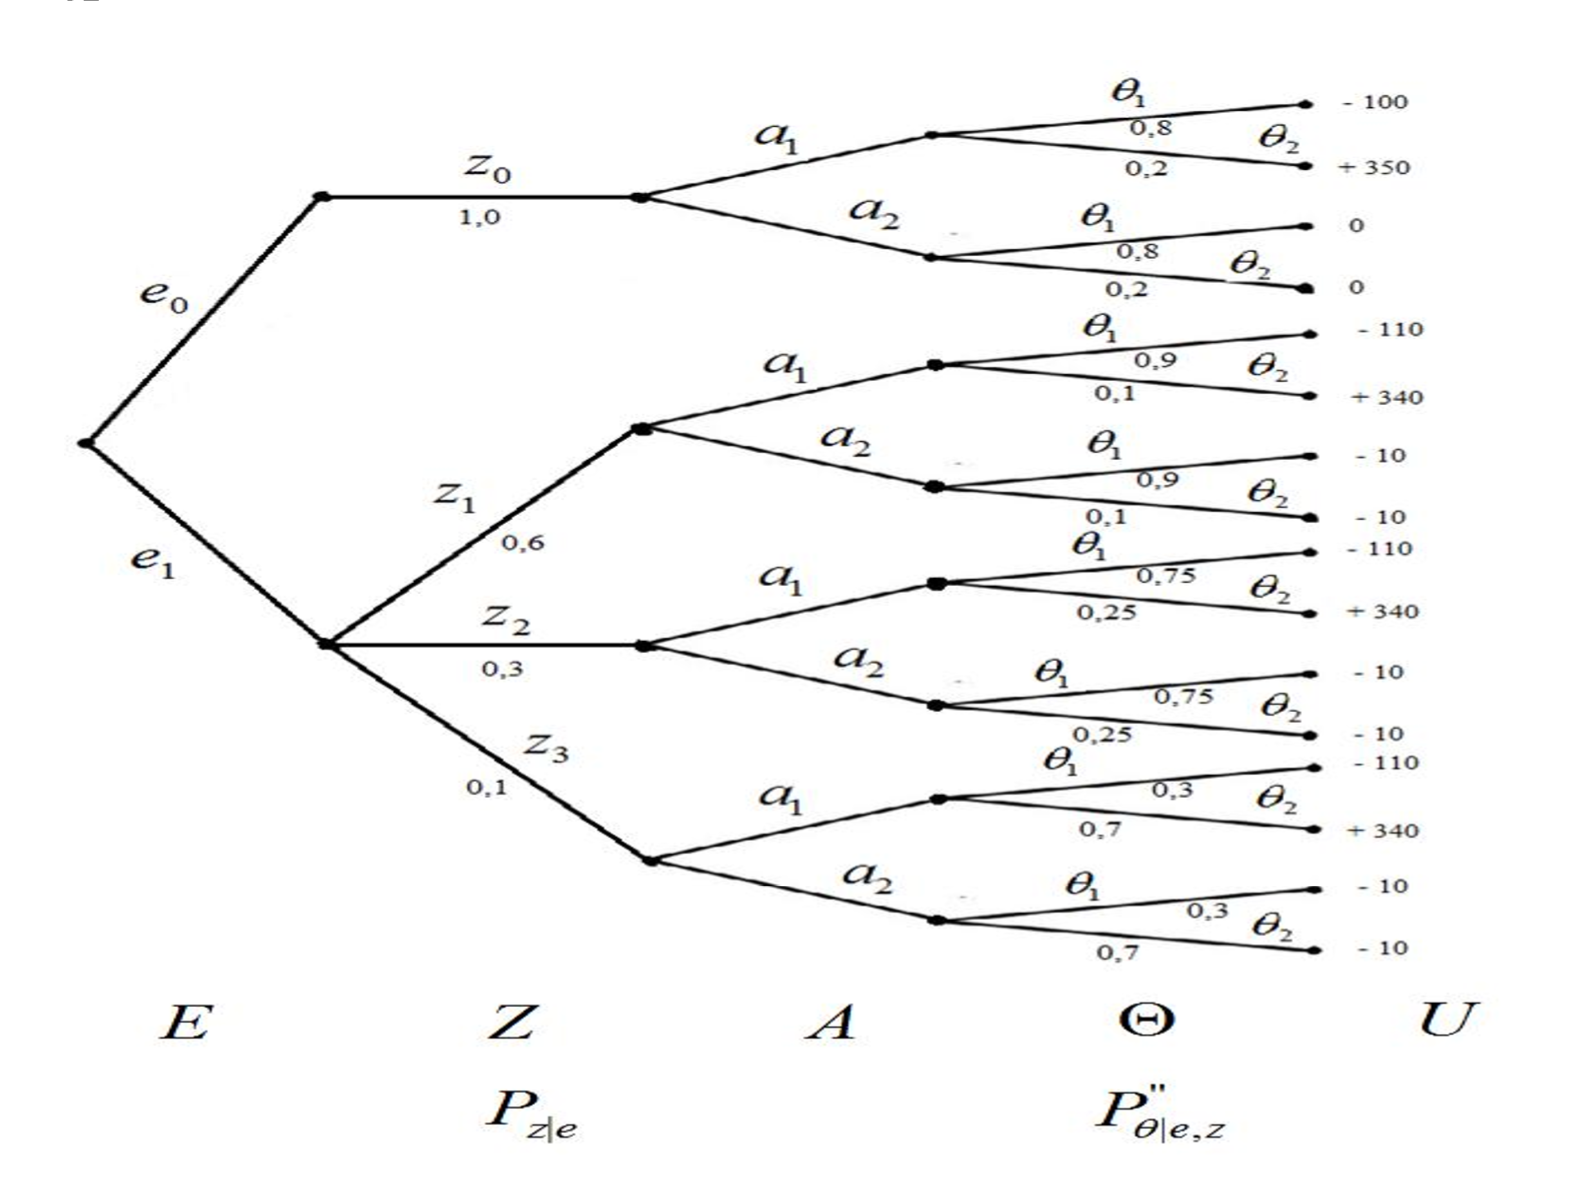
\includegraphics[width=\linewidth]{tree}
    \caption{Диаграмма дерева узлов системы}
    \label{fig:tree}
\end{figure}

Детализируем основной процесс системы, изображенный на рисунке
\ref{fig:context-diagram}. Результат изображен на рисунке \ref{fig:detailed-main-process}.

\begin{figure}[H]
    \centering
    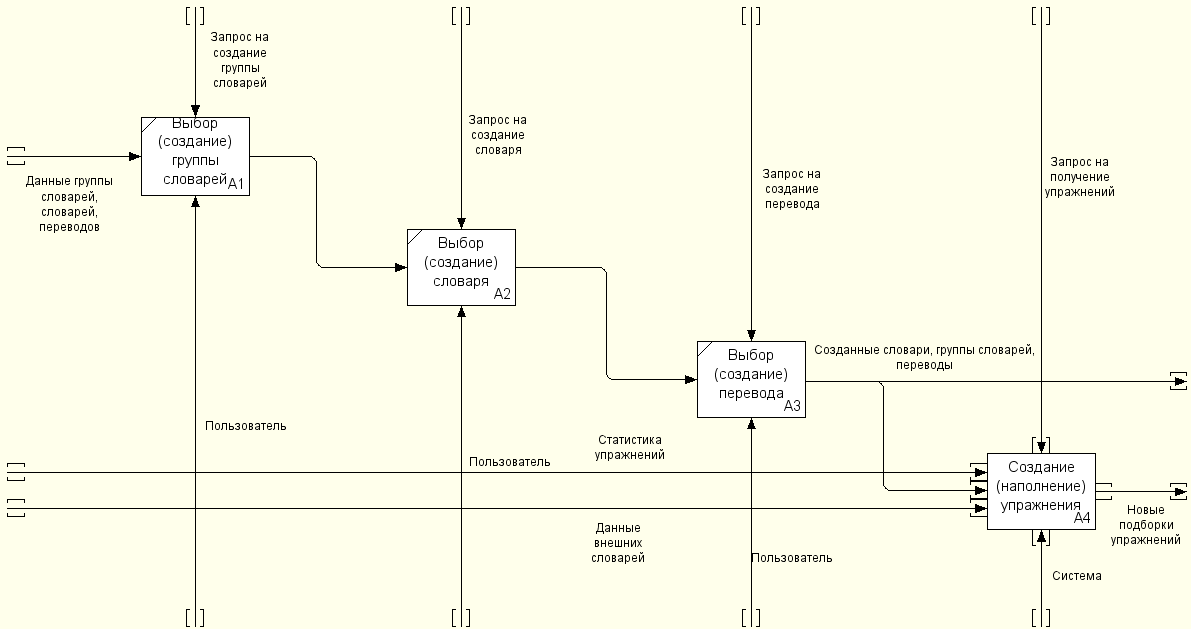
\includegraphics[width=\linewidth]{detailed-main-process}
    \caption{Детализированный основной процесс}
    \label{fig:detailed-main-process}
\end{figure}

Далее детализируем процесс создания упражнений \ref{fig:detailed-excercise-receival-process}:
\begin{figure}[H]
    \centering
    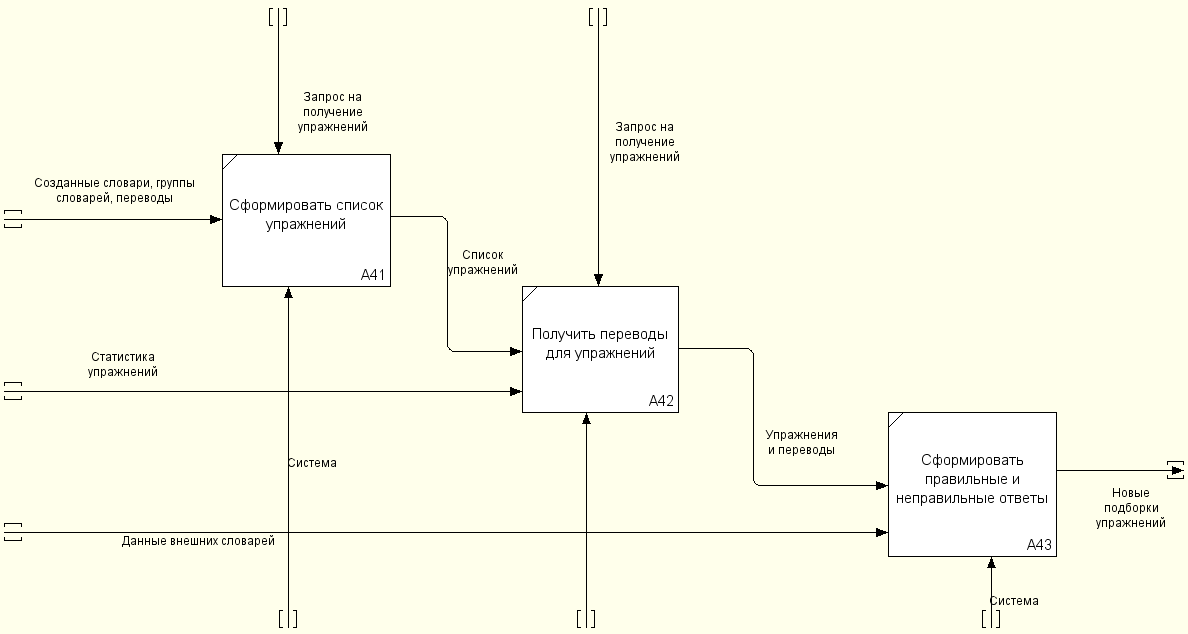
\includegraphics[width=\linewidth]{detailed-excercise-receival-process}
    \caption{Детализированный процесс создания упражнений}
    \label{fig:detailed-excercise-receival-process}
\end{figure}

\subsubsection{Модель IDEF1X}
Список потенциальных сущностей:

\begin{itemize}
    \item \textbf{Группа словарей.} Содержит информацию о группе словарей.
          Словари делятся на группы для классификации.
    \item \textbf{Словарь.} Содержит информацию о словаре. Используется для
          хранения переводов.
    \item \textbf{Перевод.} Содержит перевод: переводимое слово (выражение,
          предложение), его выбранные переводы, флеш-карточку (контекстную
          информацию).
    \item \textbf{Единица перевода.} Содержит одну единицу перевода (на родном
          языке) для того, чтобы переводы могли содержать список таких единиц.
    \item \textbf{Выбранный перевод.} Содержит связь между сущностями
          \enquote{Единица перевода} и \enquote{Перевод}.
    \item \textbf{Пользователь.} Содержит информацию о пользователе системы.
    \item \textbf{Тип упражнения.} Содержит все возможные типы упражнений.
    \item \textbf{Упражнение.} Содержит информацию о том, какое упражнение
          пользователь выполняет (выполнил), список вариантов ответа и 
    \item \textbf{Ответ пользователя при упражнении.} Содержит информацию об
          ответе пользователя при прохождении упражнения по переводу.
    \item \textbf{Экспорт группы словарей.} Содержит информацию о том, какому
          пользователю был предоставлен доступ к каким словарям или группам
          словарей.
\end{itemize}

Атрибуты сущностей:

\begin{itemize}
    \item \textbf{Группа словарей.} Id, дата удаления, Id пользователя, название, описание.
    \item \textbf{Словарь.} Id, дата удаления, Id группы словарей, название, описание.
    \item \textbf{Перевод.} Id, дата удаления, Id словаря, переводимое выражение, пользовательский контекс использования.
    \item \textbf{Единица перевода.} Id, название единицы перевода.
    \item \textbf{Выбранные перевод.} Id перевода, Id единицы перевода.
    \item \textbf{Пользователь.} Id, дата удаления, логин, пароль, электронная почта.
    \item \textbf{Тип упражнения.} Id, название типа упражнения.
    \item \textbf{Упражнение.} Id, Id типа упражнения, Id перевода, Id пользователя.
    \item \textbf{Ответ на упражнение.} Id, Id упражнения, Id единицы перевода, признак правильности выбора.
    \item \textbf{Экспорт группы словарей.} Id пользователя, Id группы словарей.
\end{itemize}

Описание предметной области на естественном языке:

\begin{enumerate}
    \item Каждая \textbf{группа словарей} может содержать несколько \textbf{словарей}.
    \item Каждый \textbf{словарь} может содержать несколько \textbf{переводов}.
    \item Каждый \textbf{перевод} может содержать несколько \textbf{выбранных переводов}.
    \item Каждый \textbf{выбранный перевод} относится только к одной \textbf{единице перевода}.
    \item Каждый \textbf{пользоваель} имеет несколько \textbf{групп словарей}.
    \item Каждое \textbf{упражнение} относится только к одному \textbf{типу упражнений}.
    \item Каждый \textbf{ответ на упражнение} является ответом только на одно \textbf{упражнение}.
    \item Каждый \textbf{экспорт группы словарей} относится только к одному пользователю.
    \item Каждый \textbf{экспорт группы словарей} относится только к одной группе словарей.
\end{enumerate}

Матрица отношений между сущностями:

\begin{landscape}
\begin{table}[H]
    \footnotesize
    \caption{Матрица отношений между сущностями}
    \begin{tabular}{ | p{1.9cm} | p{1.9cm} | p{1.9cm} | p{1.9cm} | p{1.9cm} | p{1.9cm} | p{1.9cm} | p{1.9cm} | p{1.9cm} | p{1.9cm} | p{1.9cm} | }
        \hline
        -- & Группа словарей & Словарь & Перевод & Выбранный перевод & Единица перевода  & Пользователь & Тип упражнения & Упражнение & Ответ на упражнение & Экспорт \\ \hline
        Группа словарей & -- & содержит (1:N) & & & & содержится (1:1) & & & & относится (1:1) \\ \hline
        Словарь & относится (1:1) & -- & содержит (1:N) & & & & & & & \\ \hline
        Перевод & & относится (1:1) & -- & содержит (1:N) & & & & содержит (1:N) & & \\ \hline
        Выбранный перевод & & & относится (1:1) & -- & относится (1:1) & & & & & \\ \hline
        Единица перевода & & & относится (1:1) & относится (1:1) & -- & & & & содержит (1:1) & \\ \hline
        Пользователь & содержит (1:N) & & & & & -- & & содержит (1:N) & & относится (1:1) \\ \hline
        Тип упражнения & & & & & & & -- & включает (1:N) & & \\ \hline
        Упражнение & & & относится (1:1) & & & & является (1:1) & -- & относится (1:1) & \\ \hline
        Ответ на упражнение & & & & & относится (1:1) & & & относится (1:1) & -- & \\ \hline
        Экспорт & относится (1:1) & & & & & относится (1:1) & & & & -- \\ \hline
    \end{tabular}
\end{table}
\pagebreak
\end{landscape}

Составленная диаграмма в нотации IDEF1X представлена на рисунке
\ref{fig:idef1x}:

\begin{figure}[H]
    \centering
    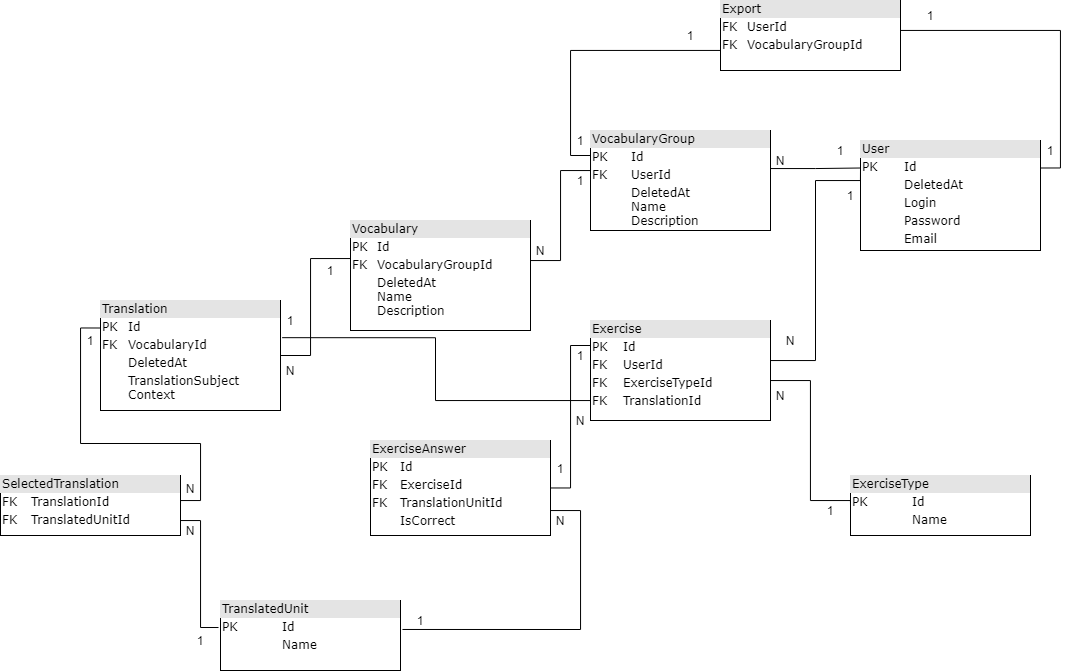
\includegraphics[width=\linewidth]{idef1x}
    \caption{Диаграмма предметной области в нотации IDEF1X}
    \label{fig:idef1x}
\end{figure}

\subsubsection{IDEF3}
\begin{table}[H]
    \caption{Список действий и объектов, составляющих моделируемый процесс}
    \begin{tabular}{| c | c |}
        \hline
        № действия & Название действия \\ \hline
        1 & Работа со словарем \\ \hline
        2 & Регистрация \\ \hline
        3 & Создание группы словарей \\ \hline
        4 & Создание словаря \\ \hline
        5 & Получение упражнений \\ \hline
        6 & Создание группы словарей \\ \hline
        7 & Формирование списка предложений \\ \hline
        8 & Получение переводов для упражнений \\ \hline
        9 & Формирование правильных и неправильных ответов \\ \hline
        10 & Получение упражнений \\ \hline
    \end{tabular}
\end{table}

\begin{table}[H]
    \caption{Список действий с указанием предшествующих и последующих слбытий с указанием типа связи}
    \begin{tabular}{| p{3cm} | p{3cm} | p{3cm} | p{3cm} | p{3cm} |}
        \hline
        № или номера предшествующего действий & Тип связи & № действия & Тип связи & № или номера последующих действий \\ \hline
         & & 1 & & \\ \hline
         & & 2 & Временное предшествование & 3,4 \\ \hline
         3,4 & Объектный поток & 5 & & \\ \hline
         & & 6 & Объектный поток & 7 \\ \hline
         7 & Объектный поток & 8,9 & Объектный поток & 10 \\ \hline
         & & 10 & & \\ \hline
    \end{tabular}
\end{table}

\begin{table}[H]
    \caption{Список действий с указанием предшествующих и последующих событий с указанием установленных отношений}
    \begin{tabular}{| p{3cm} | p{3cm} | p{3cm} | p{3cm} | p{3cm} |}
        \hline
        № или номера предшествующего действий & Вид казуального отношения & № действия & Вид казуального отношения & № или номера последующих действий \\ \hline
        2 & Асинхронный \& & 3,4 & Асинхронный \& & 5 \\ \hline
        7 & Асинхронный \& & 8,9 & Синхронный \& & 10 \\ \hline
    \end{tabular}
\end{table}

На рисунках \ref{fig:context-diagram} - \ref{fig:exercise-receival-process}
представлены разработанные диаграммы в нотации \code{IDEF3}.

\begin{figure}[H]
    \centering
    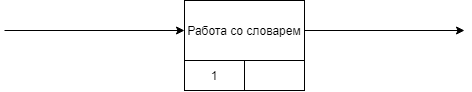
\includegraphics[width=\linewidth]{context-diagram-idef3}
    \caption{Диаграмма IDEF3 первого уровня}
    \label{fig:context-diagram}
\end{figure}

\begin{figure}[H]
    \centering
    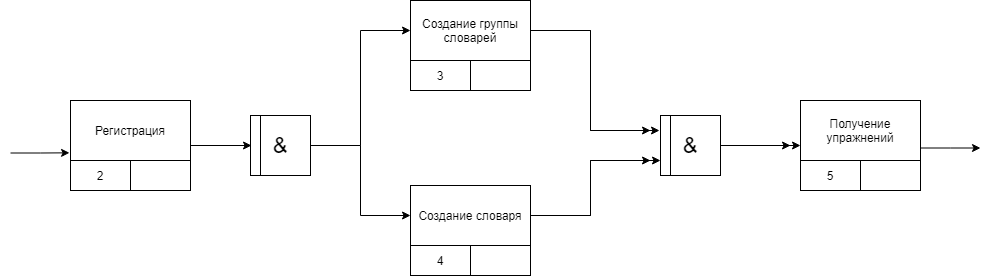
\includegraphics[width=\linewidth]{context-detailed}
    \caption{Диаграмма IDEF3 декомпозиции первого уровня}
    \label{fig:context-detailed}
\end{figure}

\begin{figure}[H]
    \centering
    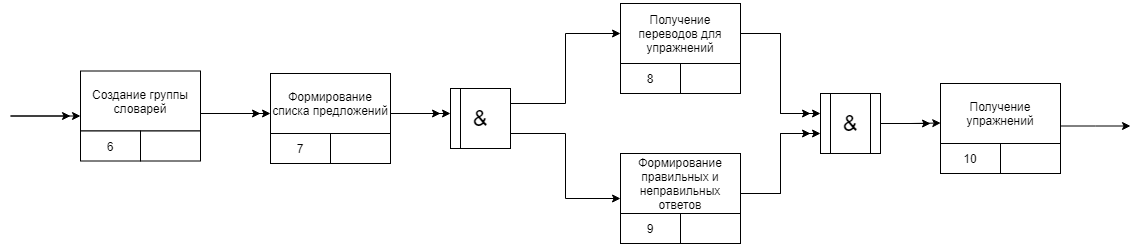
\includegraphics[width=\linewidth]{exercise-receival-process}
    \caption{Диаграмма IDEF3 декомпозиции действия 5}
    \label{fig:exercise-receival-process}
\end{figure}

\subsubsection{BPMN}
\begin{table}[H]
    \caption{Список задач, действующих лиц, объектов данных и показателей эффективности}
    \begin{tabular}{| p{2cm} | p{3cm} | p{5cm} | p{2.5cm} | p{2.5cm} |}
        \hline
        № задачи & Название задачи & № и список действий, составляющих решение задач & Участник, осуществляющий решение задачи & Объекты данных \\ \hline
        1 & Регистрация пользователя & Заполнение и отправка формы регистрации & Пользова- тель & БД Пользователей \\ \hline
        2 & Просмотр словарей & Выбор группы словарей, выбор словаря & Пользова- тель & БД словарей \\ \hline
        3 & Редактирова- ние словарей & Выбор группы словарей, выбор словаря, выбор перевода, редактирование & Пользова- тель & БД словарей \\\hline
        4 & Формирование упражнений & Выбор группы словарей или словаря & Пользова- тель & БД словарей \\ \hline
    \end{tabular}
\end{table}

Сформированная упрощенная диаграмма в нотации BPMN представлена на рисунке \ref{fig:simple}:
\begin{figure}[H]
    \centering
    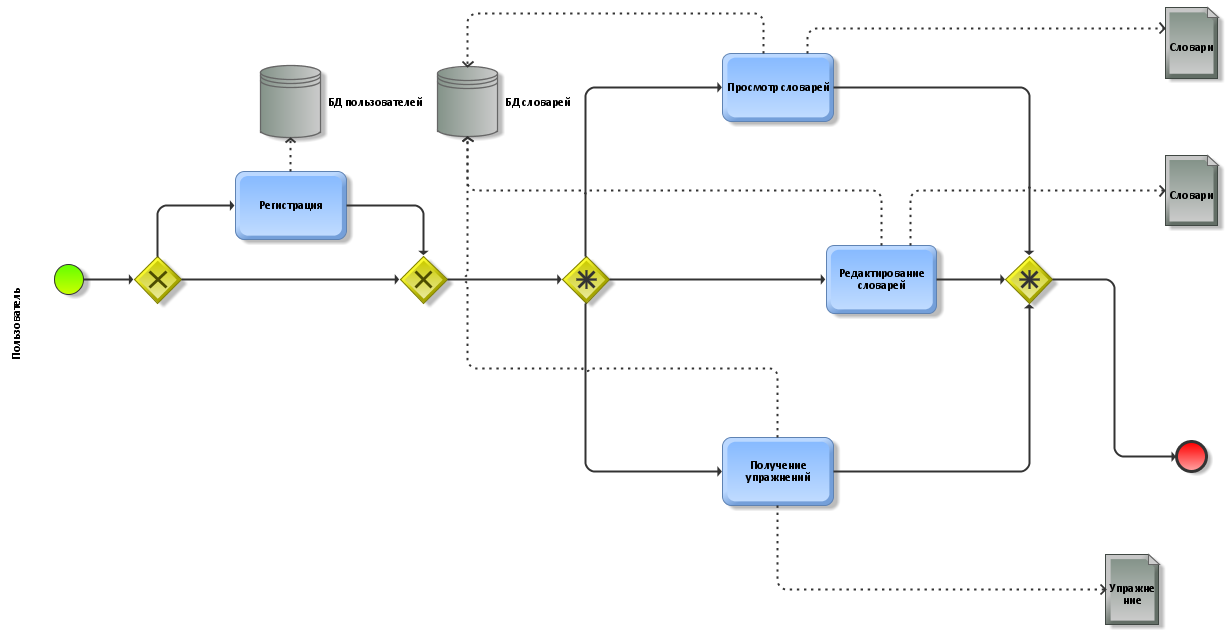
\includegraphics[width=\linewidth]{simple}
    \caption{Упрощенная диаграмма бизнес процессов в нотации BPMN}
    \label{fig:simple}
\end{figure}

Усложним модель процесса:
\begin{figure}[H]
    \centering
    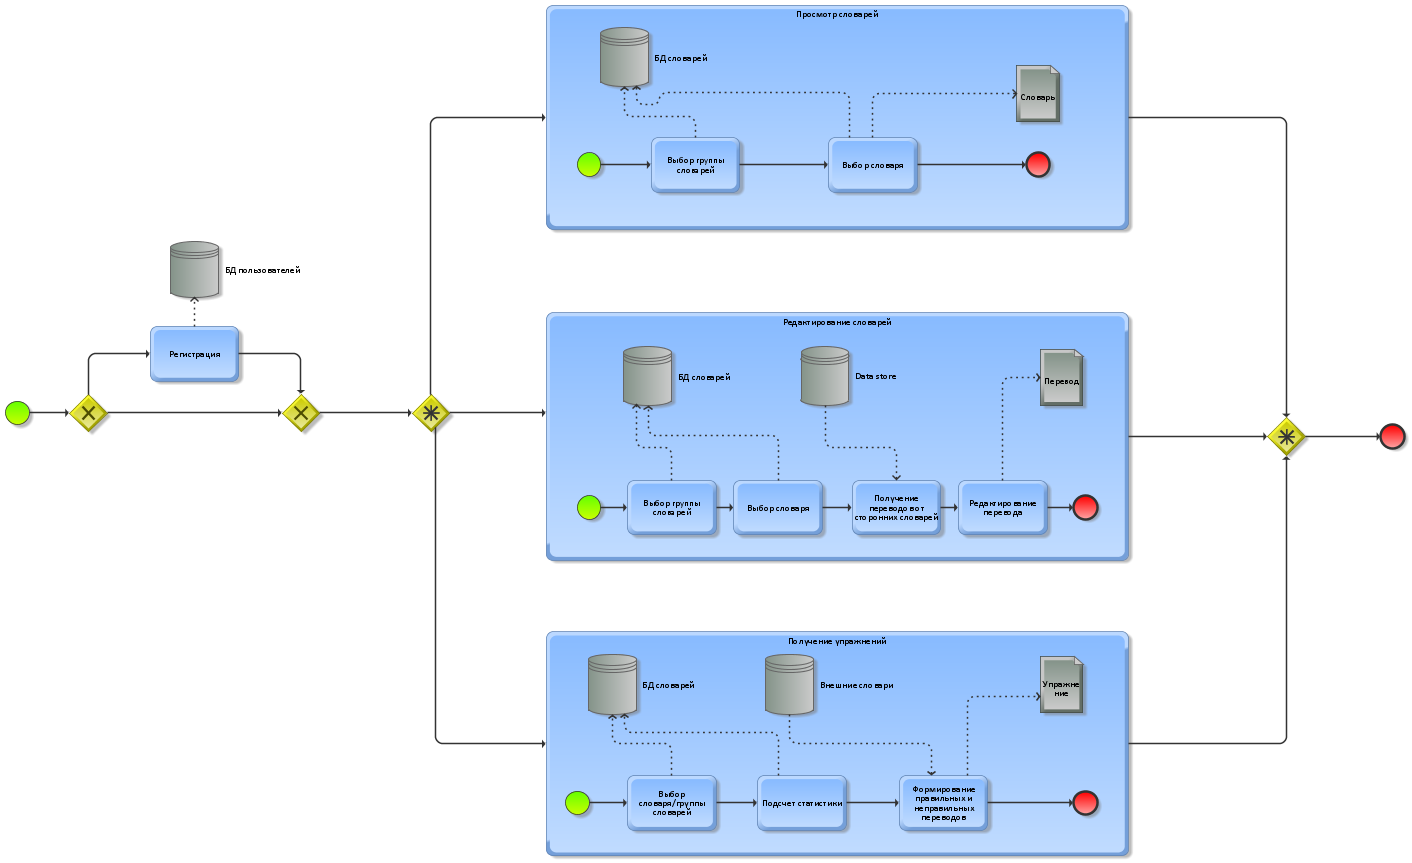
\includegraphics[width=\linewidth]{complex}
    \caption{Усложненная диаграмма бизнес процессов в нотации BPMN}
    \label{fig:complex}
\end{figure}

\section*{Заключение}
В ходе выполнения расчетно-графической работы были выбраны и применены
инструментальные средства для функционального моделирования потоков данных и
процессов, построения реляционных информационных структур, описания логики
взаимодействия информационных потоков и моделирования бизнес-процессов. Было
осуществлено исследование и функциональное моделирование процессов при помощи
DFD, IDEF0, IDEF1X, IDEF3, BPMN диаграмм.
\end{document}